\subsubsection{Proof considering $||\cdot||_2$}
We are now going to prove the theorem with the last norm we did not use yet. Let's consider the matrix $B$ with dimensions $n \times d$ and rank($B$)=$k$. This means that:
\[
    N(B) \subset \mathbb{R}^d \hspace{1cm} dim(N(B)) = d-k     
\]
If we consider matrix $V$ of the SVD decomposition of $A$:
\[
    V_{k+1} = \underbrace{\begin{bmatrix}
        \vline & \vline & \vline\\
        \underline{v_1} & \ldots & \underline{v_{k+1}}\\
        \vline & \vline & \vline
    \end{bmatrix}}_{k+1 \text{cols}}
\]
Those are the $k+1$ columns of $V$.
\[
\mathcal{C}(V_{k+1}) \subset \mathbb{R}^d  \hspace{1cm} dim(\mathcal{C}(V_{k+1})) = k+1  
\]
By adding the previous information, we have:
\[
    dim(N(B)) + dim(\mathcal{C}(V_{k+1})) = d - k + k + 1 = d + 1 
\]
Since both spaces are subset of $\mathbb{R}^d$ and their summed dimensions are $d+1$ this means that the intersection of those spaces is not empty.\\ 
\begin{center}
    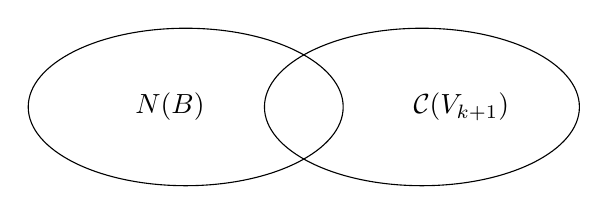
\begin{tikzpicture}
        \draw (0,0) ellipse (2cm and 1cm);
        \draw node at (-0.2,0) {$N(B)$};
        \draw (3,0) ellipse (2cm and 1cm);
        \draw node at (3.5,0) {$\mathcal{C}(V_{k+1})$};
    \end{tikzpicture}
\end{center}
Consider $\underline{w} \in N(B) \bigcap \mathcal{C}(V_{k+1})$, we suppose for easyness that $||\underline{w}||_2 = 1$.
\[
    \underline{w} = \sum_{i=1}^{k+1} c_i \underline{v_i} \overset{(\star)}{=} V_{k+1}\underline{c} \hspace{1cm} \sum_{i=1}^{k+1} c_i^2 = 1   
\]
We want to measure the following quantity:
\[
    ||A - B||^2_2 =  \underbrace{\underset{||\underline{w}||}{\sup} ||(A-B)\underline{w}||_2^2}_{\text{particular $||\underline{w}||$}} \geq \underbrace{||(A-B)\underline{w}||_2^2}_{\text{generic $||\underline{w}||$}} \implies
\]
Recall that $\underline{w} \in N(B) \implies B\underline{w} = 0$.
\[
    \implies ||A-B||^2_2 \geq ||A\underline{w}||_2^2 = \underline{w}^\intercal A^\intercal A \underline{w} \overset{\text{SVD}}{=} \underline{w}V\Sigma^\intercal \underbrace{U^\intercal U}_{I} \Sigma V^\intercal  \underline{w} = 
\] 
\[
    ? \underline{w}^\intercal V\Sigma^\intercal \Sigma V^\intercal \underline{w} \overset{(\star)}{=} \underline{c}^\intercal \underbrace{V_{k+1}^\intercal V_{k+1}}_{I} \Sigma^\intercal \Sigma  \underbrace{V_{k+1}^\intercal V_{k+1}}_{I} \underline{c} = \underline{c}^\intercal \Sigma^\intercal \Sigma \underline{c} = \sum_{i=1}^{k+1} c_i^2 \sigma_i^2 \geq    
\] 
Since singular values are ordered
\[
    \geq \sigma_{k+1}^2 \underbrace{\sum_{i=1}^{k+1} c_i^2} = \sigma_{k+1}^2    
\]
So
\[
    ||A-B||_2^2 \geq \sigma_{k+1}^2 = ||A - A_k||_2^2    
\]
And, erasing the squares:
\[
    ||A - B||_2^2 \geq \sigma_{k+1} = ||A - A_k||_2        
\]
Where $A_k$ is the rank $k$ truncated SVD approximation, therefore
\[
    ||A - A_k||_2 \leq ||A - B||_2 \hspace{1cm} \forall B \text{ of rank } k
\]


\section{PCA}
Here is a first real-world application of the SVD. PCA has the same aim as SVD i.e. find a way of projecting the dataset in a new space where variances are maximized and covariances are minimized. 

We start from $A \in \mathbb{R}^{n \times d}$ and we follow these points:
\begin{enumerate}[i]
    \item \textbf{Center the matrix \emph{A}}\\
    $\bar{A}$ is the mean centered with respect to columns while $H$ is called the centering matrix and is obtained as follows:
    \[
        H = I_n - \dfrac{1}{n} \underline{\mathbbm{1}}_n \underline{\mathbbm{1}}_n^\intercal
    \]
    Where $\underline{\mathbbm{1}}_n$ is the vector of dimension $n$ containing all ones. The centered matrix is obtained:
    \[
        \bar{A} = HA    
    \]
    \item Build the covariance matrix
    \[
        S = \dfrac{\bar{A}^\intercal \bar{A}}{n - 1}     
    \]
    Where the denominator is $n-1$ is because we want an unbiased estimator and it's not $n$ because we have already taken 1 degree of freedom by centering the matrix. The covariance matrix is semidefinite positive so we can use eigenvalues and eigenvectors decomposition.
    \[
        SV = VD \implies VDV^\intercal, D = V^\intercal SV    
    \]
    If you order the eigenvalues in decreasing order the corresponding eigenvectors are called principal components. To notice the relationship between SVD and PCA we can write:
    \[
        S = \dfrac{1}{n-1}\bar{A}^\intercal \bar{A} = \dfrac{1}{n-1} V\Sigma^\intercal U^\intercal U \Sigma V^\intercal = \dfrac{1}{n-1} V \Sigma^2 V^\intercal    
    \]
    \[
        D = \dfrac{1}{n-1}\Sigma^2 \implies \lambda_k \dfrac{\sigma_k^2}{n-1}    
    \]
\end{enumerate}
PCA is SVD applied to a particular matrix.


\subsection{Choose rank of truncated SVD}
When using truncated SVD, how to choose the rank $k$? One possibility is to use $k$ such that a predefined percentage of the variance is retained. Another idea starts from:
\[
    A = A_{true} + \gamma A_{noise}    
\]
Where: 
\begin{itemize}
    \item $A$: is out dataset
    \item $A_{true}$: is the underlying low-rank representation of our data
    \item $\gamma$: magnitude of the noise
    \item $A_{noise}$: is a gaussian noise with 0 mean and unitary variance
\end{itemize}
By defining $\tau$ as threshold we have that if $sigma_i > \tau$ we are picking $A_{true}$. 
There are two cases:
\begin{itemize}
    \item $\gamma$ is known, i.e. we know the magnitude of the noise:
    \begin{itemize}
        \item if $A \in \mathbb{R}^{n \times n}$ (square) then $\tau = \dfrac{4}{\sqrt{3}}\gamma \sqrt{n}$
        \item if $A \in \mathbb{R}^{m \times n}$ we have two more cases:
        \begin{itemize}
            \item if $n \ll m \implies \tau = \lambda(\beta)$ where $\beta = \dfrac{n}{m}$ and $\lambda$ is the following function:
            \[
                \lambda(\beta) = \sqrt{2(\beta + 1) + \dfrac{8\beta}{(\beta+1)+\sqrt{(\beta^2 + 14\beta + 1))}}}    
            \]
            \item if $m \ll n \implies \tau = \lambda(\beta)$ where $\beta = \dfrac{m}{n}$ so it's equal as before but in this case the numerator and denumerator of $\beta$ are swapped.
        \end{itemize}
    \end{itemize}
    \item $\gamma$ is unknown. We define $\tau$ as follows:
    \[
        \tau = \omega(\beta)\sigma_{med} \hspace{1cm} \omega(\beta) = \dfrac{\lambda(\beta)}{\mu_{\beta}}    
    \]
    In which $\sigma_{med}$ is the median of the singular values and $\mu_{\beta}$ is the median of the Marcenko-Pastur distribution. $\lambda(\beta)$ is the same function as before. In particular:
    \[
        \mu_{\beta} = \int_{(1-\beta)^2}^{\mu_{\beta}} \dfrac{\sqrt{((1- \sqrt{\beta})^2 - t)(t - (1- \sqrt{\beta})^2)}}{2\pi t} dt = \dfrac{1}{2}    
    \]
\end{itemize}


\subsection{Randomize SVD}
\begin{tikzpicture}
    \
\end{tikzpicture}